 
\chapter{Cochran's Formula and Omitted-Variable Bias}
 \label{chapter::cochran-ovb}
 
 
\section{Cochran's formula} 
 
 Consider an $n\times 1$ vector $Y$, an $n\times k$ matrix $X_1$, and an $n\times l$ matrix $X_2$. Similar to the FWL theorem, we do not impose any statistical models. 
We can fit the following OLS:
\begin{eqnarray}
Y &=& X_1 \hat{\beta}_1 + X_2 \hat{\beta}_2+ \hat{\varepsilon},  \label{eq::cochran-1} \\
Y &=& X_2 \tilde{\beta}_2 + \tilde{\varepsilon} ,\label{eq::cochran-2} \\
X_1 &=& X_2 \hat{\delta} + \hat{U}, \label{eq::cochran-3} 
\end{eqnarray}
where $\hat{\varepsilon}, \tilde{\varepsilon}$ are the residual vectors, and $\hat{U}$ is the residual matrix. 
The last OLS fit means the OLS fit of each column of $X_1$ on $X_2$, and therefore the corresponding residual $\hat{U}$ is an $n\times k$ matrix.
 

 \begin{theorem}
 \label{thm::cochran-formula}
 Under the OLS fits \eqref{eq::cochran-1}--\eqref{eq::cochran-3}, we have 
 $$
\tilde{\beta}_2 = \hat{\beta}_2 +  \hat{\delta} \hat{\beta}_1.
$$
 \end{theorem}
 
This is a pure linear algebra fact similar to the FWL theorem. It is called {\it Cochran's formula} in statistics. Sir David Cox \citep{cox2007generalization} attributed the formula to \citet{cochran1938omission} although Cochran himself attributed the formula to \citet{fisher1925statistical}. 


Cochran's formula may seem familiar to readers knowing the chain rule in calculus. In a deterministic world with scalar $y, x_1, x_2$, if
$$
y(x_1, x_2) = x_1  \beta_1 + x_2  \beta_2
$$
and
$$
x_1(x_2) = x_2  \delta,
$$
then
\begin{eqnarray*}
\frac{  \text{d} y }{  \text{d}x_2 } 
&=&   \frac{  \partial y }{ \partial x_1 }   \frac{  \partial x_1 }{ \partial x_2 }  + \frac{  \partial y }{ \partial x_2 }  \\
&=&  \delta   \beta_1 + \beta_2. 
\end{eqnarray*}
But the OLS decompositions above do not establish any deterministic relationships among $Y$ and $(X_1, X_2)$. 


 In some sense, the formula is obvious. From the first and the third OLS fits, we have
\begin{align} 
Y & =X_{1}\hat{\beta}_{1}+X_{2}\hat{\beta}_{2}+\hat{\varepsilon}  \nonumber  \\
 & =\left(X_{2}\hat{\delta}+\hat{U}\right)\hat{\beta}_{1}+X_{2}\hat{\beta}_{2}+\hat{\varepsilon}  \nonumber\\
 & =X_{2}\hat{\delta}\hat{\beta}_{1}+\hat{U}\hat{\beta}_{1}+X_{2}\hat{\beta}_{2}+\hat{\varepsilon}  \nonumber\\
 & =X_{2}\left(\hat{\delta}\hat{\beta}_{1}+\hat{\beta}_{2}\right)+\left(\hat{U}\hat{\beta}_{1}+\hat{\varepsilon}\right).
 \label{eq::cochran-proof1}
\end{align} 
This suggests that $\tilde{\beta}_{2}=\hat{\beta}_{2}+\hat{\delta}\hat{\beta}_{1}$. The above derivation follows from simple algebraic manipulations and does not use any properties of the OLS. To prove Theorem \ref{thm::cochran-formula}, we need to verify that the last line is indeed the OLS fit of $Y$ on $X_2.$ The proof is fact very simple. 
 
 
 \begin{myproof}{Theorem}{\ref{thm::cochran-formula}}
Based on the above discussion, 
we only need to show that \eqref{eq::cochran-proof1} is the OLS fit of $Y$
on $X_{2}$, which is equivalent to show that $\hat{U}\hat{\beta}_{1}+\hat{\varepsilon}$
is orthogonal to all columns of $X_{2}.$ This follows from
\[
X_{2}^{\T}\left(\hat{U}\hat{\beta}_{1}+\hat{\varepsilon}\right)=X_{2}^{\T}\hat{U}\hat{\beta}_{1}+X_{2}^{\T}\hat{\varepsilon}=0,
\]
because $X_{2}^{\T}\hat{U}=0$ based on the OLS fit in \eqref{eq::cochran-3} and $X_{2}^{\T}\hat{\varepsilon}=0$
based on the OLS fit in \eqref{eq::cochran-1}. 
\end{myproof}



Figure \ref{fig::cochranformula} illustrates Theorem \ref{thm::cochran-formula}. Intuitively, $\tilde{\beta}_{2}$  measures the total impact of $X_2$ on $Y$, which has two channels: $\hat{\beta}_{2}$ measures the impact acting directly and $\hat{\delta}\hat{\beta}_{1}$ measures the impact acting indirectly through $X_1$. 



\begin{figure}
\centering
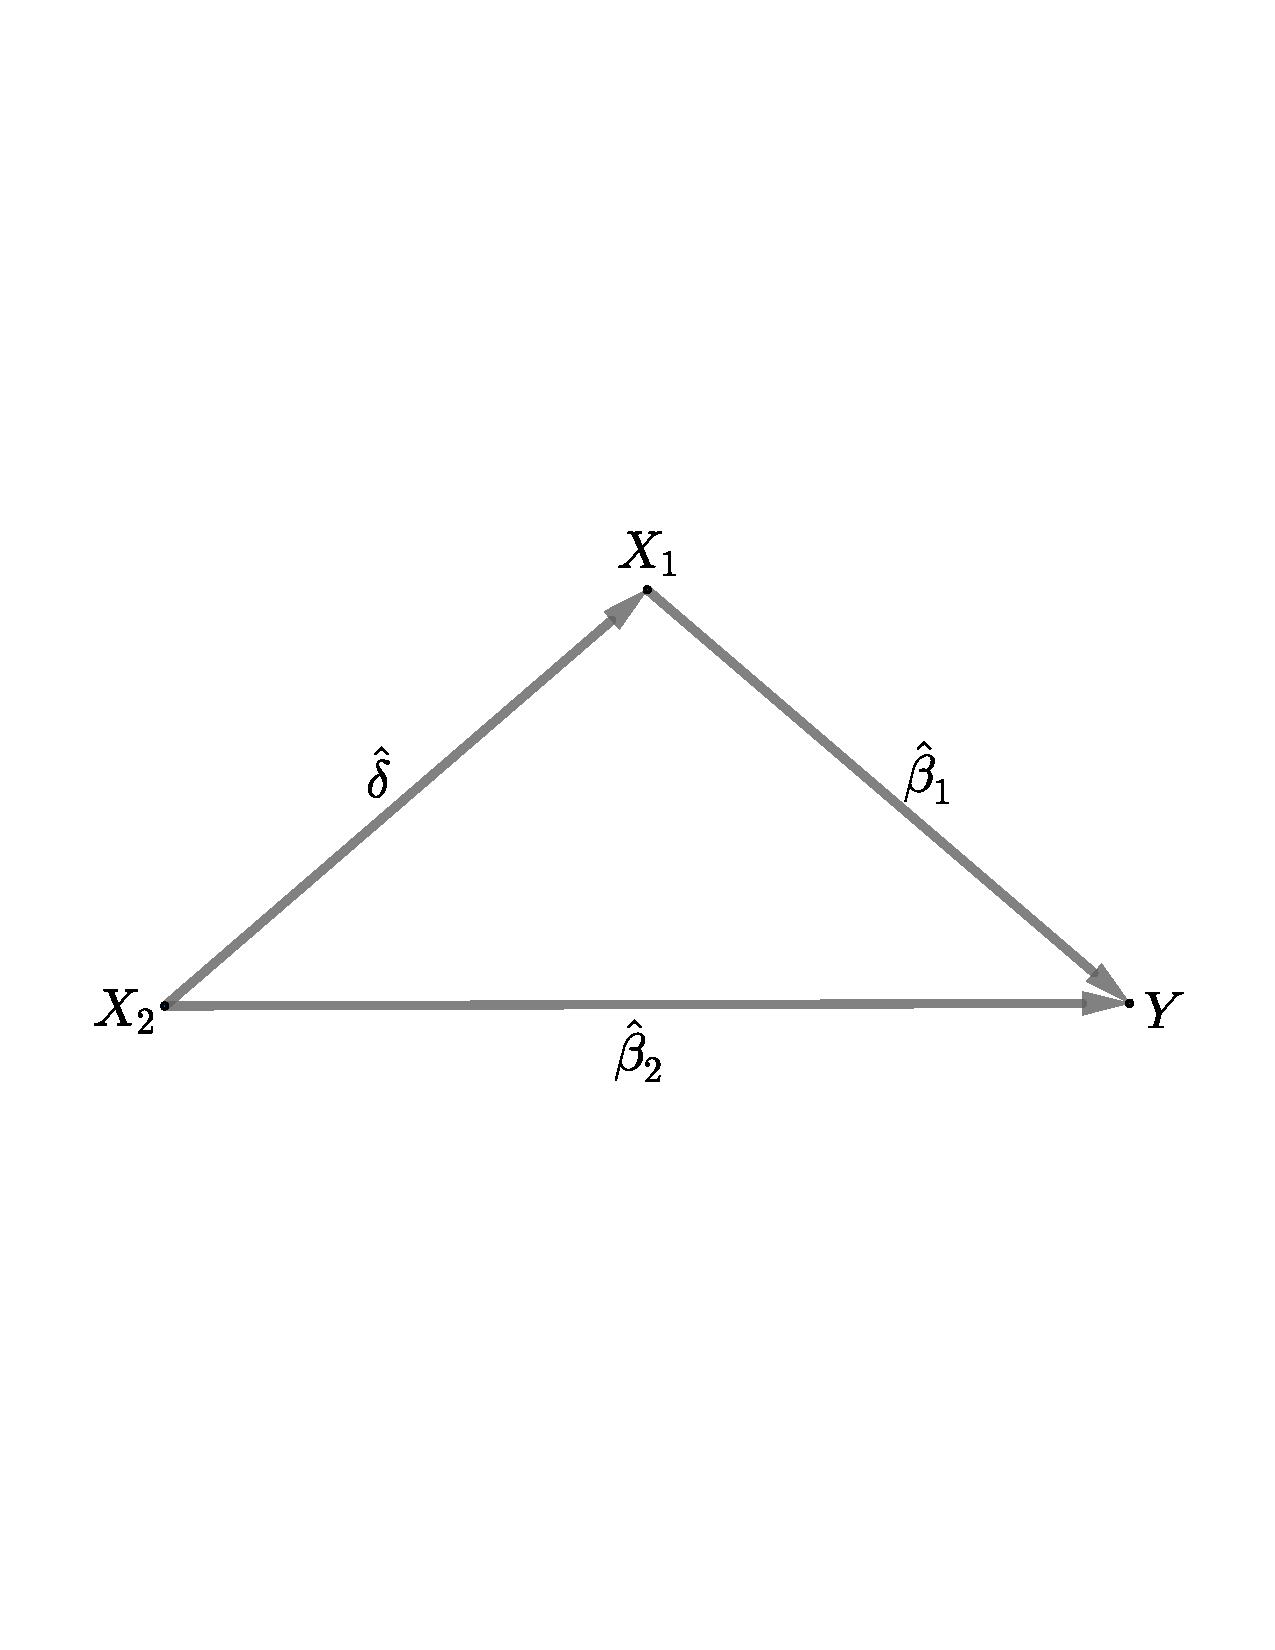
\includegraphics[width = 0.7\textwidth]{figures/cochrangraph.pdf}
\caption{A diagram for Cochran's formula}\label{fig::cochranformula}
\end{figure} 



Figure \ref{fig::cochranformula} shows the interplay among three variables. Theoretically, we can discuss a system of more than three variables which is called the {\it path model}. This more advanced topic is beyond the scope of this book. \citet{sewall1921correlation, wright1934method}'s initial discussion of this approach was motivated by genetic studies. See \citet{freedman2009statistical} for a textbook introduction. 



 
\section{Omitted-variable bias} 
\label{sec::ovb}


The proof of Theorem \ref{thm::cochran-formula} is very simple. However, it is one of the most insightful formulas in statistics. Econometricians often call it the {\it omitted-variable bias} formula because it quantifies the bias of the OLS coefficient of $X_2$ in the short regression omitting possibly important variables in $X_1$.  If the OLS coefficient from the long regression is unbiased then the the OLS coefficient from the short regression has a biased term
$
 \hat{\delta} \hat{\beta}_1,
$
which equals the product of the coefficient of $X_2$ in the OLS fit of $X_1$ on $X_2$ and the coefficient of $X_1$ in the long regression. 



Below I will discuss a canonical example of using OLS to estimate the treatment effect in observational studies. For unit $i\  (i = 1, \ldots, n)$, let $y_i$ be the outcome, $z_i$ be the binary treatment indicator ($1$ for the treatment group and $0$ for the control group) and $x_i$ be the observed covariate vector. Practitioners often fit the following OLS:
$$
y_i = \tilde{\beta}_0 + \tilde{\beta}_1 z_i + \tilde{\beta}^{\T}_2 x_i + \tilde{\varepsilon}_i
$$
and interpret $ \tilde{\beta}_1$ as the treatment effect estimate. However, observational studies may suffer from unmeasured confounding, that is, the treatment and control units differ in unobserved but important ways. In the simplest case, the above OLS may have omitted a variable $u_i$ for each unit $i$, which is called a {\it confounder}. The oracle OLS is
$$
y_i = \hat{\beta}_0 + \hat{\beta}_1 z_i + \hat{\beta}^{\T}_2 x_i  + \hat{\beta}_3 u_i + \hat{\varepsilon}_i
$$
and the coefficient $ \hat{\beta}_1$ is an unbiased estimator if the model with $u_i$ is correct. 
With $X_1$ containing the values of the $u_i$'s and $X_2$ containing the values of the $(1, z_i, x_i^{\T})$'s, Cochran's formula implies that
$$
\begin{pmatrix}
\tilde{\beta}_0 \\
 \tilde{\beta}_1 \\
  \tilde{\beta}_2
\end{pmatrix}
=
\begin{pmatrix}
\hat{\beta}_0 \\
 \hat{\beta}_1 \\
  \hat{\beta}_2
\end{pmatrix}
+ 
\hat{\beta}_3 \begin{pmatrix}
 \hat{\delta}_0 \\
 \hat{\delta}_1 \\
  \hat{\delta}_2
\end{pmatrix}
$$
where $(  \hat{\delta}_0,  \hat{\delta}_1, \hat{\delta}_2^{\T})^{\T}$ is the coefficient vector in the OLS fit of $u_i$ on $(1, z_i, x_i)$. Therefore, we can
quantify the difference between the observed estimate $ \tilde{\beta}_1$ and oracle estimate $ \hat{\beta}_1$:
$$
\tilde{\beta}_1  - \hat{\beta}_1 =  \hat{\beta}_3 \hat{\delta}_1,
$$
which is sometimes called the {\it confounding bias}. 

Using the basic properties of OLS, we can show that $\hat{\delta}_1$ equals the difference in means of $e_i =  u_i -   \hat{\delta}_2^{\T} x_i$ across the treatment and control groups:
$$
\hat{\delta}_1 = \bar{e}_1 - \bar{e}_0,
$$
where the bar and subscript jointly denote the sample mean of a particular variable within a treatment group.
So
\begin{eqnarray} \label{eq::sensitivity-1}
\tilde{\beta} - \hat{\beta}_1 =  \hat{\beta}_3  ( \bar{e}_1 - \bar{e}_0).
\end{eqnarray} 
Moreover, we can obtain a more explicit formula for $\hat{\delta}_1$: 
$$
\hat{\delta}_1 = \bar{u}_1 - \bar{u}_0 -  \hat{\delta}_2^{\T}  ( \bar{x}_1 - \bar{x}_0 ).
$$
So
\begin{eqnarray} \label{eq::sensitivity-2}
\tilde{\beta} - \hat{\beta}_1 =  \hat{\beta}_3(\bar{u}_1 - \bar{u}_0) -  \hat{\beta}_3\hat{\delta}_2^{\T}  ( \bar{x}_1 - \bar{x}_0 ).
\end{eqnarray} 

Both \eqref{eq::sensitivity-1} and \eqref{eq::sensitivity-2} give some insights into the bias due to omitting an important covariate $u$. It is clear that the bias depends on $ \hat{\beta}_3$, which quantifies the relationship between $u$ and $y$. The formula \eqref{eq::sensitivity-1} shows that the bias also depends on the imbalance in means of $u$ across the treatment and control groups, after adjusting for the observed covariates $x$, that is, the imbalance in means of the residual confounding. The formula \eqref{eq::sensitivity-2} shows a more explicit formula of the bias. The above discussion is often called {\it bias analysis} in epidemiology or {\it sensitivity analysis} in statistics and econometrics. 




\section{Homework problems}


\paragraph{Baron--Kenny method for mediation analysis}
\label{hw07::baron-kenney}

The Baron--Kenny method, popularized by \citet{baron1986moderator}, is one of the most cited methods in social science. 
It concerns the interplay among three variables $z, m, y$ controlling for some other variables $x$. Let $Z, M, Y$ be  $n\times 1$ vectors representing the observed values of $z, m, y$, and let $X$ be the $n\times p$ matrix representing the observations of $x$. The question of interest is to assess the ``direct'' and ``indirect'' effects of $z$ on $y$, acting independently and through $m$, respectively. We do not need to define these notions precisely since we are only interested in the algebraic property below. 


The Baron--Kenny method runs the OLS
$$
Y = \hat{\beta}_0 1_n   +  \hat{\beta}_1 Z  + \hat{\beta}_2 M  + X \hat{\beta}_3 + \hat{\varepsilon}_Y
$$
and interprets $\hat{\beta}_1$ as the estimator of the ``direct effect'' of $z$ on $y$. 
The ``indirect effect'' of $z$ on $y$ through $m$ has two estimators. First, based on the OLS
$$
Y = \tilde{\beta}_0 1_n   +  \tilde{\beta}_1 Z     + X \tilde{\beta}_3 + \tilde{\varepsilon}_Y,
$$
define the {\it difference estimator} as 
$
 \tilde{\beta}_1 -   \hat{\beta}_1 .
$
Second, based on the OLS
$$
M = \hat{\gamma}_0 1_n   +  \hat{\gamma}_1 Z    + X \hat{\gamma}_2 + \hat{\varepsilon}_M , 
$$
define the {\it product estimator} as
$
  \hat{\gamma}_1   \hat{\beta}_2 .
$
Figure \ref{fig::bkmethod} illustrates the OLS fits used in defining the estimators. 

\begin{figure}
\centering
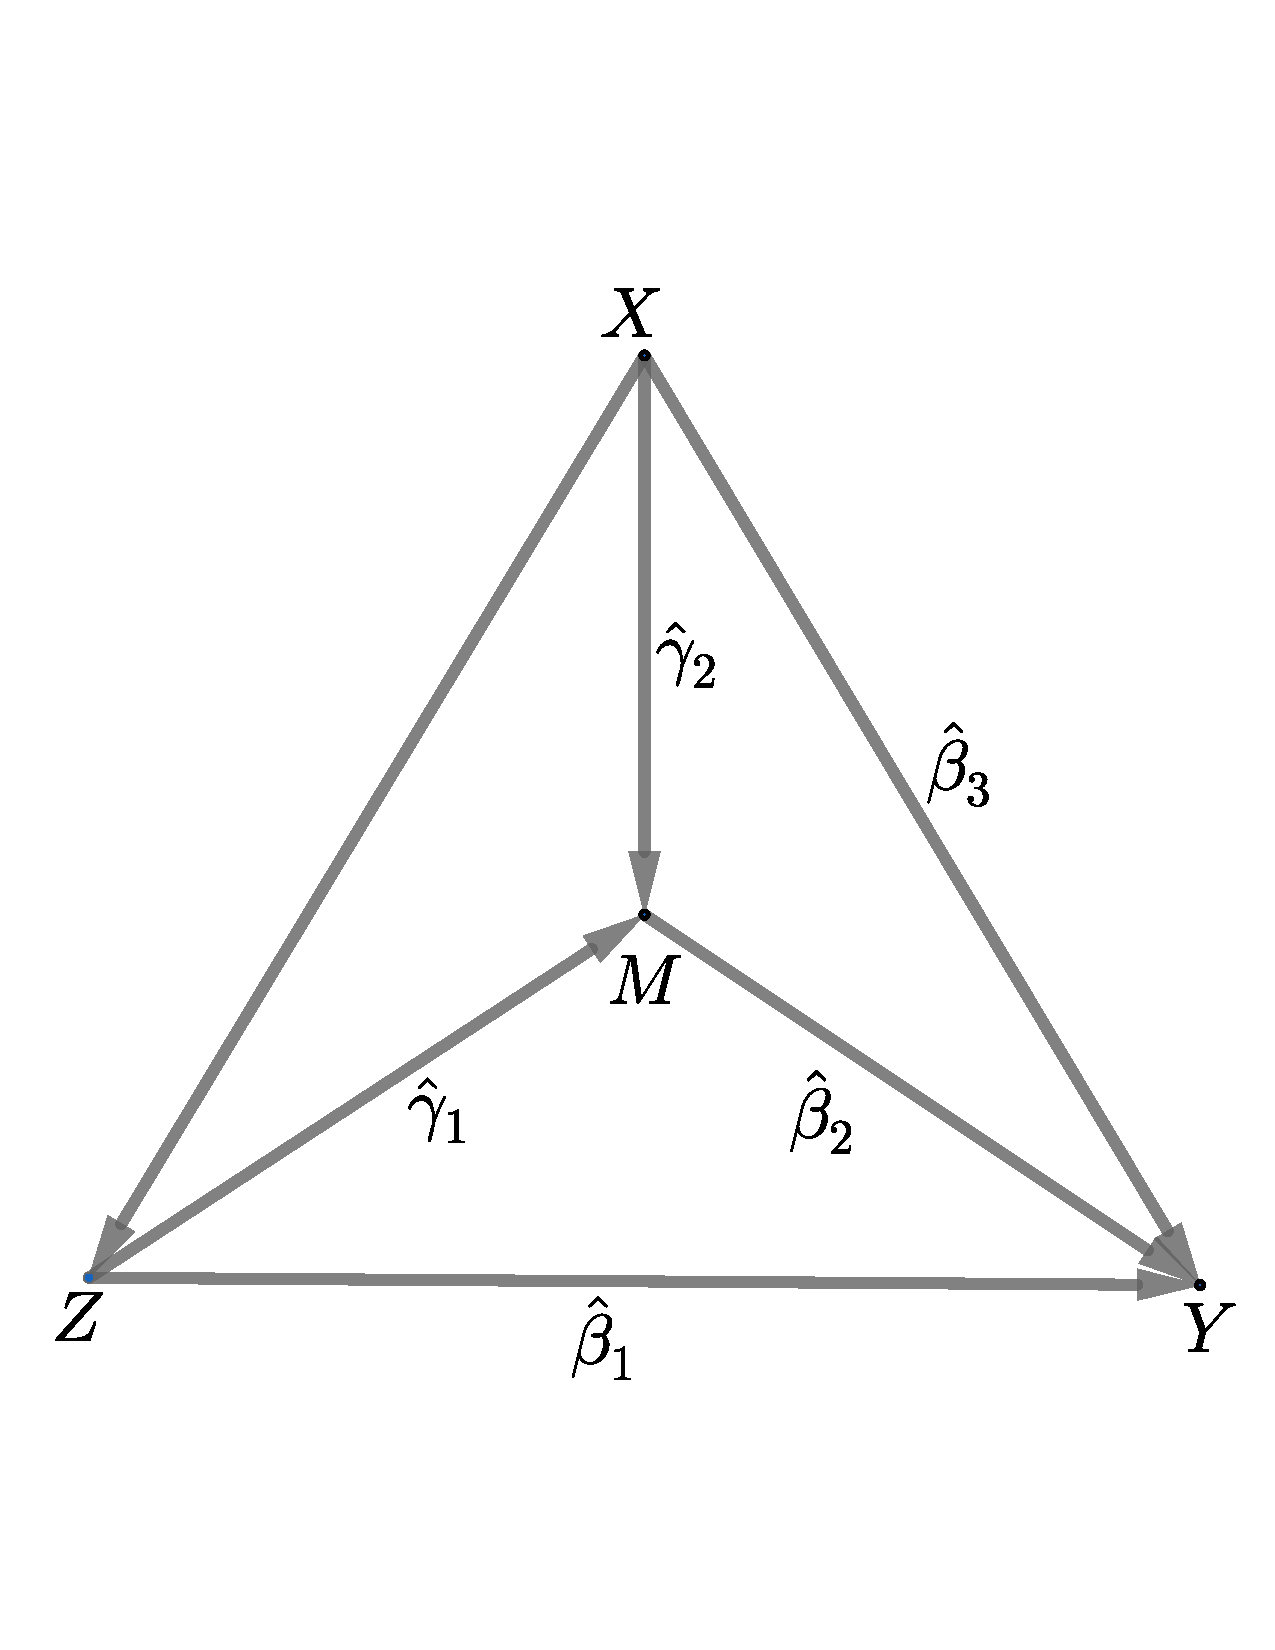
\includegraphics[width = 0.5\textwidth]{figures/baronkennygraph.pdf}
\caption{The graph for the Baron--Kenny method}\label{fig::bkmethod}
\end{figure} 


Prove that 
$$ 
\tilde{\beta}_1 -   \hat{\beta}_1 =    \hat{\gamma}_1   \hat{\beta}_2
$$ 
that is, the difference estimator and product estimator are numerically identical. 



\paragraph{A special case of path analysis}\label{hw07cochran::path}



Figure \ref{fig::path} represents the order of the variables $X_1, X_2, X_3, Y \in \mathbb{R}^n$. Run the following OLS:
\begin{eqnarray*}
Y &=& \hat{\beta}_0 1_n  + \hat{\beta}_1 X_1 + \hat{\beta}_2 X_2 + \hat{\beta}_3 X_3 + \hat{\varepsilon}_Y, \\
X_3 &=&   \hat{\delta}_0 1_n+ \hat{\delta}_1 X_1 + \hat{\delta}_2 X_2 +  \hat{\varepsilon}_3, \\
X_2 &=&  \hat{\theta}_0 1_n+ \hat{\theta}_1 X_1 +  \hat{\varepsilon}_2,
\end{eqnarray*}
and
$$
Y = \tilde{\beta}_0 1_n+ \tilde{\beta}_1 X_1 + \tilde{\varepsilon}_Y.
$$
Show that 
$$
 \tilde{\beta}_1 =  \hat{\beta}_1  +  \hat{\beta}_2\hat{\theta}_1  +  \hat{\beta}_3 \hat{\delta}_1 +  \hat{\beta}_3 \hat{\delta}_2  \hat{\theta}_1 .
$$

Remark: The OLS coefficient of $X_1$ in the short regression of $Y$ on $(1_n, X_1)$ equals the summation of all the path coefficients from $X_1$ to $Y$ as illustrated by Figure \ref{fig::path}. This problem is a special case of the path model, but the conclusion holds in general. 

\begin{figure}
\centering
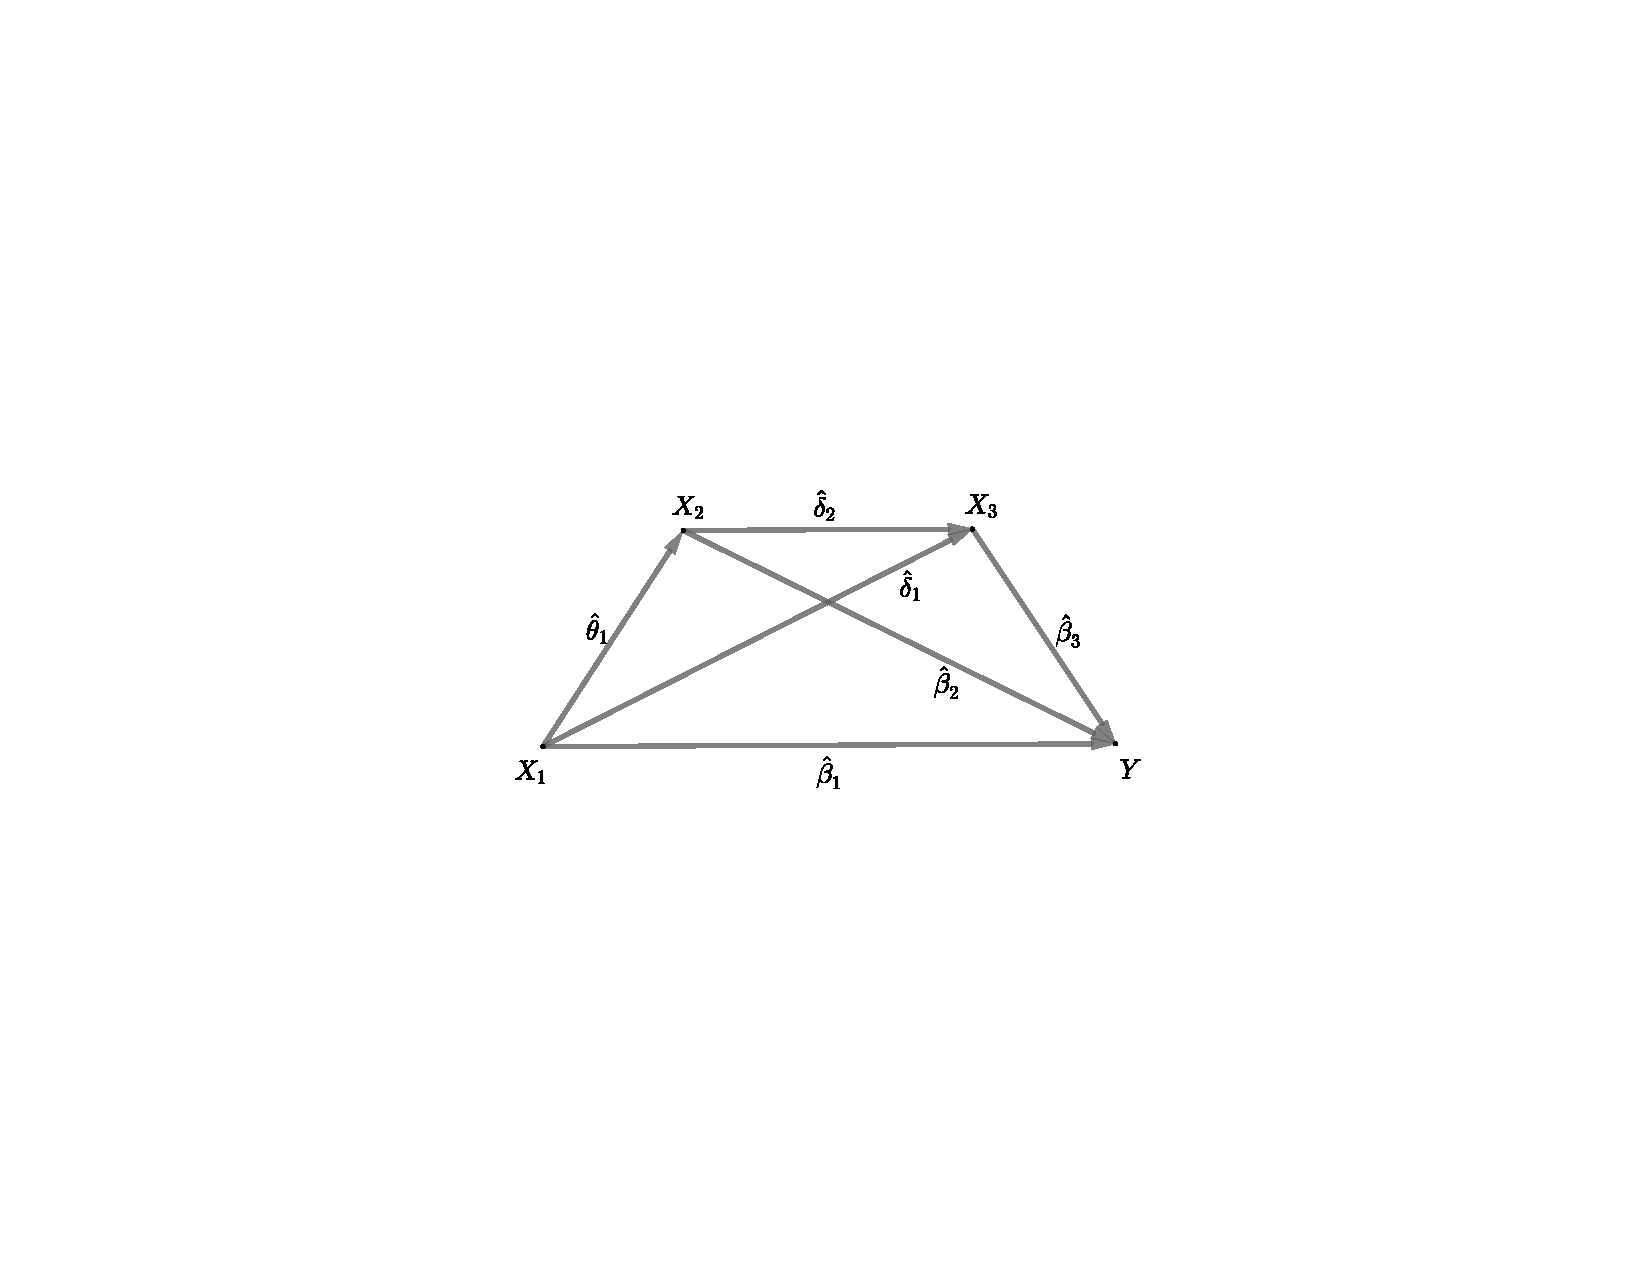
\includegraphics[width = 0.8\textwidth]{figures/path_cochran.pdf}
\caption{A path model}\label{fig::path}
\end{figure} 






  \paragraph{EHW in long and short regressions}\label{hw08::ehw-long-short-ols}
Theorem \ref{thm::cochran-formula} gives Cochran's formula related to the coefficients from three OLS fits. 
This problem concerns the covariance estimation. 
There are at least two ways to estimate the covariance of $\tilde \beta_2$ in the short regression \eqref{eq::cochran-2}. First, from the second OLS fit, the EHW covariance estimator is
$$
\tilde V_2 = (X_2^{\T} X_2)^{-1}   X_2^{\T}  \text{diag}(\tilde \varepsilon^2)  X_2 (X_2^{\T} X_2)^{-1}.
$$
Second, Cochran's formula implies that 
$$
\tilde \beta_2 = (\hat \delta, I_l)  \begin{pmatrix}
\hat{\beta}_1 \\
\hat{\beta}_2
\end{pmatrix}
$$ is a linear transformation of the coefficient from the long regression, which further justifies the EHW covariance estimator 
$$
\tilde V_2 ' = (\hat \delta, I_l) (X^{\T} X)^{-1}   X^{\T}  \text{diag}(\hat \varepsilon^2)  X (X^{\T} X)^{-1}  \begin{pmatrix}
\hat \delta^{\T} \\
I_l
\end{pmatrix} .
$$

Show that 
$$
\tilde V_2 ' = (X_2^{\T} X_2)^{-1}   X_2^{\T}  \text{diag}(\hat \varepsilon^2)  X_2 (X_2^{\T} X_2)^{-1}.
$$


Hint: Use the result in Problem \ref{hw6::inverse-block-gram}. 

Remark: Based on Theorem \ref{thm::fwl-se}, the EHW covariance estimator for $\hat{\beta}_2$ is
$$
\hat{V}_2 = (\tilde X_2^{\T} \tilde X_2)^{-1}   \tilde X_2^{\T}  \text{diag}(\hat \varepsilon^2)  \tilde X_2 (\tilde X_2^{\T} \tilde X_2)^{-1},
$$
where $ \tilde X_2 = (I_n - H_1) X_2$. 

 
 
 \paragraph{Statistical properties of under-fitted OLS}
\label{hw::underfit-ols}


Assume that $Y = X \beta + \varepsilon = X_1 \beta_1 + X_2 \beta_2 + \varepsilon$ follows the Gauss--Markov model, where $X_1 \in \mathbb{R}^{n\times k}$, $X_2 \in \mathbb{R}^{n\times l}$, and $\cov(\varepsilon)=\sigma^2 I_n$. However, we only fit the OLS of $Y$ on $X_2$ with coefficient $\tilde{\beta}_2$ and estimated variance $\tilde{\sigma}^2$. Show that
$$
E(\tilde{\beta}_2) =  (X_2^{\T} X_2)^{-1} X_2^{\T} X_1 \beta_1 +   \beta_2 ,\quad
\var( \tilde{\beta}_2) = \sigma^2 (X_2^{\T} X_2)^{-1}
$$
and
$$
E(\tilde{\sigma}^2) = \sigma^2 + \beta_1^{\T} X_1^{\T} (I_n - H_2) X_1\beta_1/(n-l) \geq \sigma^2 . 
$$
 
 

